\documentclass[1p]{elsarticle_modified}
%\bibliographystyle{elsarticle-num}

%\usepackage[colorlinks]{hyperref}
%\usepackage{abbrmath_seonhwa} %\Abb, \Ascr, \Acal ,\Abf, \Afrak
\usepackage{amsfonts}
\usepackage{amssymb}
\usepackage{amsmath}
\usepackage{amsthm}
\usepackage{scalefnt}
\usepackage{amsbsy}
\usepackage{kotex}
\usepackage{caption}
\usepackage{subfig}
\usepackage{color}
\usepackage{graphicx}
\usepackage{xcolor} %% white, black, red, green, blue, cyan, magenta, yellow
\usepackage{float}
\usepackage{setspace}
\usepackage{hyperref}

\usepackage{tikz}
\usetikzlibrary{arrows}

\usepackage{multirow}
\usepackage{array} % fixed length table
\usepackage{hhline}

%%%%%%%%%%%%%%%%%%%%%
\makeatletter
\renewcommand*\env@matrix[1][\arraystretch]{%
	\edef\arraystretch{#1}%
	\hskip -\arraycolsep
	\let\@ifnextchar\new@ifnextchar
	\array{*\c@MaxMatrixCols c}}
\makeatother %https://tex.stackexchange.com/questions/14071/how-can-i-increase-the-line-spacing-in-a-matrix
%%%%%%%%%%%%%%%

\usepackage[normalem]{ulem}

\newcommand{\msout}[1]{\ifmmode\text{\sout{\ensuremath{#1}}}\else\sout{#1}\fi}
%SOURCE: \msout is \stkout macro in https://tex.stackexchange.com/questions/20609/strikeout-in-math-mode

\newcommand{\cancel}[1]{
	\ifmmode
	{\color{red}\msout{#1}}
	\else
	{\color{red}\sout{#1}}
	\fi
}

\newcommand{\add}[1]{
	{\color{blue}\uwave{#1}}
}

\newcommand{\replace}[2]{
	\ifmmode
	{\color{red}\msout{#1}}{\color{blue}\uwave{#2}}
	\else
	{\color{red}\sout{#1}}{\color{blue}\uwave{#2}}
	\fi
}

\newcommand{\Sol}{\mathcal{S}} %segment
\newcommand{\D}{D} %diagram
\newcommand{\A}{\mathcal{A}} %arc


%%%%%%%%%%%%%%%%%%%%%%%%%%%%%5 test

\def\sl{\operatorname{\textup{SL}}(2,\Cbb)}
\def\psl{\operatorname{\textup{PSL}}(2,\Cbb)}
\def\quan{\mkern 1mu \triangleright \mkern 1mu}

\theoremstyle{definition}
\newtheorem{thm}{Theorem}[section]
\newtheorem{prop}[thm]{Proposition}
\newtheorem{lem}[thm]{Lemma}
\newtheorem{ques}[thm]{Question}
\newtheorem{cor}[thm]{Corollary}
\newtheorem{defn}[thm]{Definition}
\newtheorem{exam}[thm]{Example}
\newtheorem{rmk}[thm]{Remark}
\newtheorem{alg}[thm]{Algorithm}

\newcommand{\I}{\sqrt{-1}}
\begin{document}

%\begin{frontmatter}
%
%\title{Boundary parabolic representations of knots up to 8 crossings}
%
%%% Group authors per affiliation:
%\author{Yunhi Cho} 
%\address{Department of Mathematics, University of Seoul, Seoul, Korea}
%\ead{yhcho@uos.ac.kr}
%
%
%\author{Seonhwa Kim} %\fnref{s_kim}}
%\address{Center for Geometry and Physics, Institute for Basic Science, Pohang, 37673, Korea}
%\ead{ryeona17@ibs.re.kr}
%
%\author{Hyuk Kim}
%\address{Department of Mathematical Sciences, Seoul National University, Seoul 08826, Korea}
%\ead{hyukkim@snu.ac.kr}
%
%\author{Seokbeom Yoon}
%\address{Department of Mathematical Sciences, Seoul National University, Seoul, 08826,  Korea}
%\ead{sbyoon15@snu.ac.kr}
%
%\begin{abstract}
%We find all boundary parabolic representation of knots up to 8 crossings.
%
%\end{abstract}
%\begin{keyword}
%    \MSC[2010] 57M25 
%\end{keyword}
%
%\end{frontmatter}

%\linenumbers
%\tableofcontents
%
\newcommand\colored[1]{\textcolor{white}{\rule[-0.35ex]{0.8em}{1.4ex}}\kern-0.8em\color{red} #1}%
%\newcommand\colored[1]{\textcolor{white}{ #1}\kern-2.17ex	\textcolor{white}{ #1}\kern-1.81ex	\textcolor{white}{ #1}\kern-2.15ex\color{red}#1	}

{\Large $\underline{11a_{108}~(K11a_{108})}$}

\setlength{\tabcolsep}{10pt}
\renewcommand{\arraystretch}{1.6}
\vspace{1cm}\begin{tabular}{m{100pt}>{\centering\arraybackslash}m{274pt}}
\multirow{5}{120pt}{
	\centering
	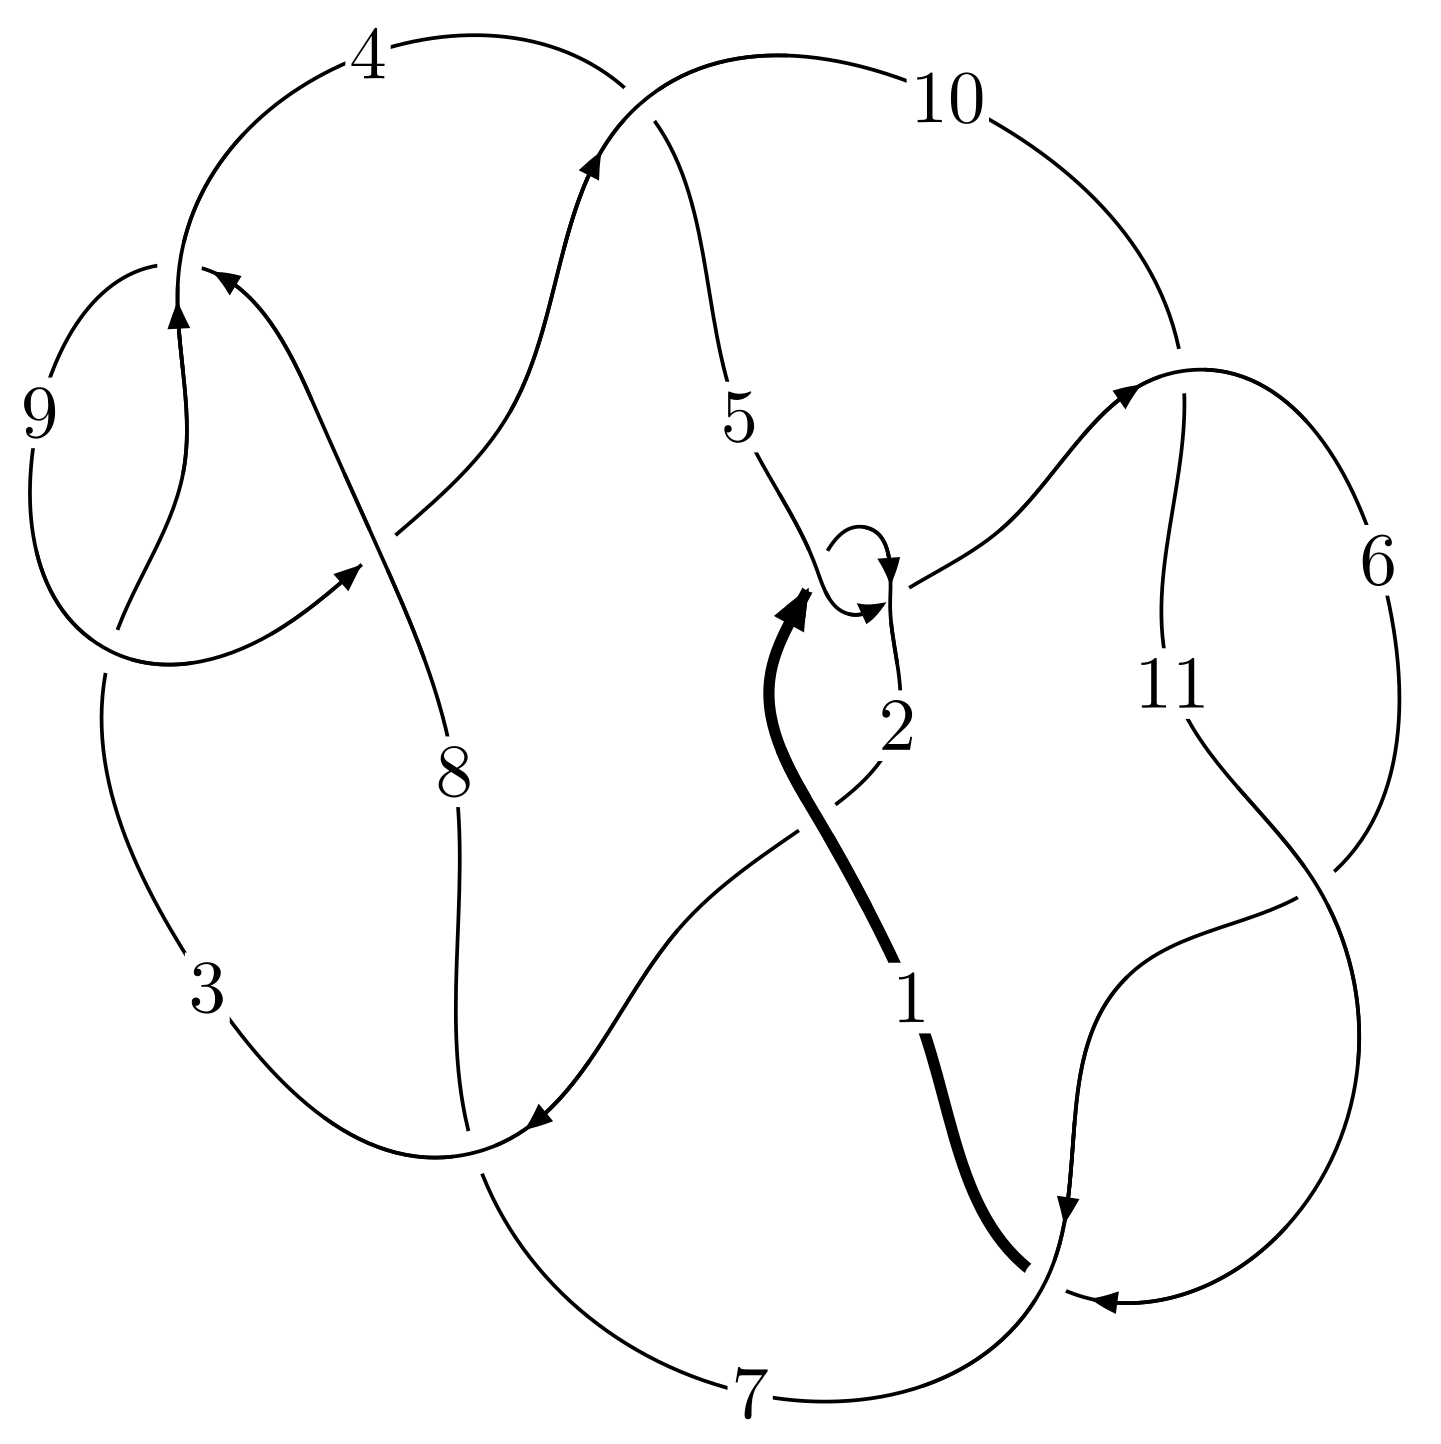
\includegraphics[width=112pt]{../../../GIT/diagram.site/Diagrams/png/357_11a_108.png}\\
\ \ \ A knot diagram\footnotemark}&
\allowdisplaybreaks
\textbf{Linearized knot diagam} \\
\cline{2-2}
 &
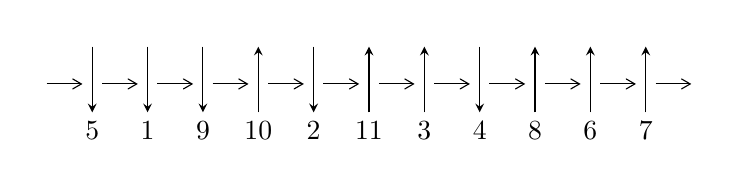
\begin{tikzpicture}[x=20pt, y=17pt]
	% nodes
	\node (C0) at (0, 0) {};
	\node (C1) at (1, 0) {};
	\node (C1U) at (1, +1) {};
	\node (C1D) at (1, -1) {5};

	\node (C2) at (2, 0) {};
	\node (C2U) at (2, +1) {};
	\node (C2D) at (2, -1) {1};

	\node (C3) at (3, 0) {};
	\node (C3U) at (3, +1) {};
	\node (C3D) at (3, -1) {9};

	\node (C4) at (4, 0) {};
	\node (C4U) at (4, +1) {};
	\node (C4D) at (4, -1) {10};

	\node (C5) at (5, 0) {};
	\node (C5U) at (5, +1) {};
	\node (C5D) at (5, -1) {2};

	\node (C6) at (6, 0) {};
	\node (C6U) at (6, +1) {};
	\node (C6D) at (6, -1) {11};

	\node (C7) at (7, 0) {};
	\node (C7U) at (7, +1) {};
	\node (C7D) at (7, -1) {3};

	\node (C8) at (8, 0) {};
	\node (C8U) at (8, +1) {};
	\node (C8D) at (8, -1) {4};

	\node (C9) at (9, 0) {};
	\node (C9U) at (9, +1) {};
	\node (C9D) at (9, -1) {8};

	\node (C10) at (10, 0) {};
	\node (C10U) at (10, +1) {};
	\node (C10D) at (10, -1) {6};

	\node (C11) at (11, 0) {};
	\node (C11U) at (11, +1) {};
	\node (C11D) at (11, -1) {7};
	\node (C12) at (12, 0) {};

	% arrows
	\draw[->,>={angle 60}]
	(C0) edge (C1) (C1) edge (C2) (C2) edge (C3) (C3) edge (C4) (C4) edge (C5) (C5) edge (C6) (C6) edge (C7) (C7) edge (C8) (C8) edge (C9) (C9) edge (C10) (C10) edge (C11) (C11) edge (C12) ;	\draw[->,>=stealth]
	(C1U) edge (C1D) (C2U) edge (C2D) (C3U) edge (C3D) (C4D) edge (C4U) (C5U) edge (C5D) (C6D) edge (C6U) (C7D) edge (C7U) (C8U) edge (C8D) (C9D) edge (C9U) (C10D) edge (C10U) (C11D) edge (C11U) ;
	\end{tikzpicture} \\
\hhline{~~} \\& 
\textbf{Solving Sequence} \\ \cline{2-2} 
 &
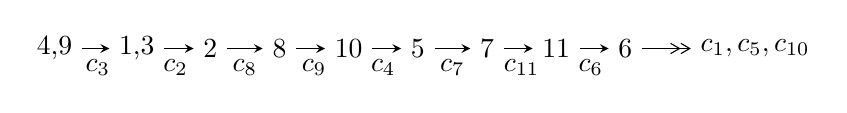
\begin{tikzpicture}[x=25pt, y=7pt]
	% node
	\node (A0) at (-1/8, 0) {4,9};
	\node (A1) at (17/16, 0) {1,3};
	\node (A2) at (17/8, 0) {2};
	\node (A3) at (25/8, 0) {8};
	\node (A4) at (33/8, 0) {10};
	\node (A5) at (41/8, 0) {5};
	\node (A6) at (49/8, 0) {7};
	\node (A7) at (57/8, 0) {11};
	\node (A8) at (65/8, 0) {6};
	\node (C1) at (1/2, -1) {$c_{3}$};
	\node (C2) at (13/8, -1) {$c_{2}$};
	\node (C3) at (21/8, -1) {$c_{8}$};
	\node (C4) at (29/8, -1) {$c_{9}$};
	\node (C5) at (37/8, -1) {$c_{4}$};
	\node (C6) at (45/8, -1) {$c_{7}$};
	\node (C7) at (53/8, -1) {$c_{11}$};
	\node (C8) at (61/8, -1) {$c_{6}$};
	\node (A9) at (10, 0) {$c_{1},c_{5},c_{10}$};

	% edge
	\draw[->,>=stealth]	
	(A0) edge (A1) (A1) edge (A2) (A2) edge (A3) (A3) edge (A4) (A4) edge (A5) (A5) edge (A6) (A6) edge (A7) (A7) edge (A8) ;
	\draw[->>,>={angle 60}]	
	(A8) edge (A9);
\end{tikzpicture} \\ 

\end{tabular} \\

\footnotetext{
The image of knot diagram is generated by the software ``\textbf{Draw programme}" developed by Andrew Bartholomew(\url{http://www.layer8.co.uk/maths/draw/index.htm\#Running-draw}), where we modified some parts for our purpose(\url{https://github.com/CATsTAILs/LinksPainter}).
}\phantom \\ \newline 
\centering \textbf{Ideals for irreducible components\footnotemark of $X_{\text{par}}$} 
 
\begin{align*}
I^u_{1}&=\langle 
-4 u^{40}+4 u^{39}+\cdots+4 b+4,\;-2 u^{40}+4 u^{39}+\cdots+4 a-2,\;u^{41}-2 u^{40}+\cdots-4 u+2\rangle \\
I^u_{2}&=\langle 
46 u^4 a^2+10 u^4 a+\cdots-33 a+56,\\
\phantom{I^u_{2}}&\phantom{= \langle  }-2 u^3 a^2- u^4 a-2 a^2 u^2+2 u^3 a+3 u^4+a^3-2 a^2 u+u^2 a+u^3-2 a^2+a u+2 u^2+2 a+3 u+1,\\
\phantom{I^u_{2}}&\phantom{= \langle  }u^5+u^4+2 u^3+u^2+u+1\rangle \\
I^u_{3}&=\langle 
u^3+b+u-1,\;u^3-2 u^2+2 a-4,\;u^4+2 u^2+2\rangle \\
\\
I^v_{1}&=\langle 
a,\;b+1,\;v-1\rangle \\
\end{align*}
\raggedright * 4 irreducible components of $\dim_{\mathbb{C}}=0$, with total 61 representations.\\
\footnotetext{All coefficients of polynomials are rational numbers. But the coefficients are sometimes approximated in decimal forms when there is not enough margin.}
\newpage
\renewcommand{\arraystretch}{1}
\centering \section*{I. $I^u_{1}= \langle -4 u^{40}+4 u^{39}+\cdots+4 b+4,\;-2 u^{40}+4 u^{39}+\cdots+4 a-2,\;u^{41}-2 u^{40}+\cdots-4 u+2 \rangle$}
\flushleft \textbf{(i) Arc colorings}\\
\begin{tabular}{m{7pt} m{180pt} m{7pt} m{180pt} }
\flushright $a_{4}=$&$\begin{pmatrix}1\\0\end{pmatrix}$ \\
\flushright $a_{9}=$&$\begin{pmatrix}0\\u\end{pmatrix}$ \\
\flushright $a_{1}=$&$\begin{pmatrix}\frac{1}{2} u^{40}- u^{39}+\cdots+\frac{1}{2} u+\frac{1}{2}\\u^{40}- u^{39}+\cdots+\frac{1}{2} u-1\end{pmatrix}$ \\
\flushright $a_{3}=$&$\begin{pmatrix}1\\- u^2\end{pmatrix}$ \\
\flushright $a_{2}=$&$\begin{pmatrix}-\frac{1}{4} u^{33}-2 u^{31}+\cdots-\frac{1}{2} u^3+1\\\frac{1}{4} u^{35}+\frac{9}{4} u^{33}+\cdots-\frac{3}{2} u^2-\frac{1}{2} u\end{pmatrix}$ \\
\flushright $a_{8}=$&$\begin{pmatrix}u\\u\end{pmatrix}$ \\
\flushright $a_{10}=$&$\begin{pmatrix}u^3\\u^3+u\end{pmatrix}$ \\
\flushright $a_{5}=$&$\begin{pmatrix}- u^6- u^4+1\\- u^6-2 u^4- u^2\end{pmatrix}$ \\
\flushright $a_{7}=$&$\begin{pmatrix}- u^3\\u^5+u^3+u\end{pmatrix}$ \\
\flushright $a_{11}=$&$\begin{pmatrix}-\frac{1}{4} u^{36}-\frac{9}{4} u^{34}+\cdots-\frac{1}{2} u+\frac{1}{2}\\-\frac{1}{4} u^{36}-\frac{5}{2} u^{34}+\cdots-\frac{1}{2} u^2- u\end{pmatrix}$ \\
\flushright $a_{6}=$&$\begin{pmatrix}-\frac{1}{4} u^{36}-\frac{9}{4} u^{34}+\cdots-\frac{1}{2} u+\frac{1}{2}\\\frac{1}{4} u^{38}+\frac{5}{2} u^{36}+\cdots+u^3+u\end{pmatrix}$\\ \flushright $a_{6}=$&$\begin{pmatrix}-\frac{1}{4} u^{36}-\frac{9}{4} u^{34}+\cdots-\frac{1}{2} u+\frac{1}{2}\\\frac{1}{4} u^{38}+\frac{5}{2} u^{36}+\cdots+u^3+u\end{pmatrix}$\\&\end{tabular}
\flushleft \textbf{(ii) Obstruction class $= -1$}\\~\\
\flushleft \textbf{(iii) Cusp Shapes $= 2 u^{40}-4 u^{39}+22 u^{38}-40 u^{37}+114 u^{36}-196 u^{35}+364 u^{34}-604 u^{33}+786 u^{32}-1280 u^{31}+1188 u^{30}-1918 u^{29}+1256 u^{28}-1996 u^{27}+904 u^{26}-1290 u^{25}+434 u^{24}-232 u^{23}+184 u^{22}+468 u^{21}+136 u^{20}+520 u^{19}+84 u^{18}+194 u^{17}+4 u^{16}-120 u^{15}-4 u^{14}-258 u^{13}+52 u^{12}-234 u^{11}+84 u^{10}-128 u^9+90 u^8-30 u^7+64 u^6+2 u^5+24 u^4-10 u^3-4 u^2-2 u$}\\~\\
\newpage\renewcommand{\arraystretch}{1}
\flushleft \textbf{(iv) u-Polynomials at the component}\newline \\
\begin{tabular}{m{50pt}|m{274pt}}
Crossings & \hspace{64pt}u-Polynomials at each crossing \\
\hline $$\begin{aligned}c_{1},c_{5}\end{aligned}$$&$\begin{aligned}
&u^{41}+2 u^{40}+\cdots+5 u-1
\end{aligned}$\\
\hline $$\begin{aligned}c_{2}\end{aligned}$$&$\begin{aligned}
&u^{41}+14 u^{40}+\cdots+u+1
\end{aligned}$\\
\hline $$\begin{aligned}c_{3},c_{8}\end{aligned}$$&$\begin{aligned}
&u^{41}+2 u^{40}+\cdots-4 u-2
\end{aligned}$\\
\hline $$\begin{aligned}c_{4},c_{7}\end{aligned}$$&$\begin{aligned}
&u^{41}-2 u^{40}+\cdots-24 u-16
\end{aligned}$\\
\hline $$\begin{aligned}c_{6},c_{10},c_{11}\end{aligned}$$&$\begin{aligned}
&u^{41}-2 u^{40}+\cdots-7 u-1
\end{aligned}$\\
\hline $$\begin{aligned}c_{9}\end{aligned}$$&$\begin{aligned}
&u^{41}-22 u^{40}+\cdots+8 u+4
\end{aligned}$\\
\hline
\end{tabular}\\~\\
\newpage\renewcommand{\arraystretch}{1}
\flushleft \textbf{(v) Riley Polynomials at the component}\newline \\
\begin{tabular}{m{50pt}|m{274pt}}
Crossings & \hspace{64pt}Riley Polynomials at each crossing \\
\hline $$\begin{aligned}c_{1},c_{5}\end{aligned}$$&$\begin{aligned}
&y^{41}-14 y^{40}+\cdots+y-1
\end{aligned}$\\
\hline $$\begin{aligned}c_{2}\end{aligned}$$&$\begin{aligned}
&y^{41}+34 y^{40}+\cdots+737 y-1
\end{aligned}$\\
\hline $$\begin{aligned}c_{3},c_{8}\end{aligned}$$&$\begin{aligned}
&y^{41}+22 y^{40}+\cdots+8 y-4
\end{aligned}$\\
\hline $$\begin{aligned}c_{4},c_{7}\end{aligned}$$&$\begin{aligned}
&y^{41}-34 y^{40}+\cdots-16448 y-256
\end{aligned}$\\
\hline $$\begin{aligned}c_{6},c_{10},c_{11}\end{aligned}$$&$\begin{aligned}
&y^{41}-46 y^{40}+\cdots-47 y-1
\end{aligned}$\\
\hline $$\begin{aligned}c_{9}\end{aligned}$$&$\begin{aligned}
&y^{41}-6 y^{40}+\cdots+160 y-16
\end{aligned}$\\
\hline
\end{tabular}\\~\\
\newpage\flushleft \textbf{(vi) Complex Volumes and Cusp Shapes}
$$\begin{array}{c|c|c}  
\text{Solutions to }I^u_{1}& \I (\text{vol} + \sqrt{-1}CS) & \text{Cusp shape}\\
 \hline 
\begin{aligned}
u &= -0.503278 + 0.876227 I \\
a &= -1.01864 - 1.35377 I \\
b &= -0.184951 - 0.697202 I\end{aligned}
 & -1.85795 + 5.19311 I & -2.06190 - 8.35313 I \\ \hline\begin{aligned}
u &= -0.503278 - 0.876227 I \\
a &= -1.01864 + 1.35377 I \\
b &= -0.184951 + 0.697202 I\end{aligned}
 & -1.85795 - 5.19311 I & -2.06190 + 8.35313 I \\ \hline\begin{aligned}
u &= \phantom{-}0.595879 + 0.924278 I \\
a &= -1.261860 + 0.541147 I \\
b &= -0.683532 + 0.365288 I\end{aligned}
 & \phantom{-}3.43135 - 8.38206 I & \phantom{-}3.46275 + 8.23571 I \\ \hline\begin{aligned}
u &= \phantom{-}0.595879 - 0.924278 I \\
a &= -1.261860 - 0.541147 I \\
b &= -0.683532 - 0.365288 I\end{aligned}
 & \phantom{-}3.43135 + 8.38206 I & \phantom{-}3.46275 - 8.23571 I \\ \hline\begin{aligned}
u &= \phantom{-}0.012198 + 0.896132 I \\
a &= \phantom{-}1.24032 + 1.28683 I \\
b &= \phantom{-}0.765320 + 0.507138 I\end{aligned}
 & \phantom{-}1.35320 - 1.46651 I & \phantom{-}7.22861 + 4.90542 I \\ \hline\begin{aligned}
u &= \phantom{-}0.012198 - 0.896132 I \\
a &= \phantom{-}1.24032 - 1.28683 I \\
b &= \phantom{-}0.765320 - 0.507138 I\end{aligned}
 & \phantom{-}1.35320 + 1.46651 I & \phantom{-}7.22861 - 4.90542 I \\ \hline\begin{aligned}
u &= \phantom{-}0.662080 + 0.589897 I \\
a &= \phantom{-}0.314575 + 0.870590 I \\
b &= \phantom{-}0.143067 + 0.847335 I\end{aligned}
 & \phantom{-}2.46953 + 3.52956 I & \phantom{-}2.12209 - 2.66433 I \\ \hline\begin{aligned}
u &= \phantom{-}0.662080 - 0.589897 I \\
a &= \phantom{-}0.314575 - 0.870590 I \\
b &= \phantom{-}0.143067 - 0.847335 I\end{aligned}
 & \phantom{-}2.46953 - 3.52956 I & \phantom{-}2.12209 + 2.66433 I \\ \hline\begin{aligned}
u &= -0.860560 + 0.141859 I \\
a &= -0.542033 + 0.556076 I \\
b &= -0.51707 - 2.21472 I\end{aligned}
 & \phantom{-}7.79923 - 9.18843 I & \phantom{-}3.80065 + 5.17633 I \\ \hline\begin{aligned}
u &= -0.860560 - 0.141859 I \\
a &= -0.542033 - 0.556076 I \\
b &= -0.51707 + 2.21472 I\end{aligned}
 & \phantom{-}7.79923 + 9.18843 I & \phantom{-}3.80065 - 5.17633 I\\
 \hline 
 \end{array}$$\newpage$$\begin{array}{c|c|c}  
\text{Solutions to }I^u_{1}& \I (\text{vol} + \sqrt{-1}CS) & \text{Cusp shape}\\
 \hline 
\begin{aligned}
u &= \phantom{-}0.861859 + 0.085768 I \\
a &= \phantom{-}0.673275 + 0.352479 I \\
b &= \phantom{-}0.26299 - 1.41656 I\end{aligned}
 & \phantom{-}9.69240 + 2.90753 I & \phantom{-}6.01430 - 0.84016 I \\ \hline\begin{aligned}
u &= \phantom{-}0.861859 - 0.085768 I \\
a &= \phantom{-}0.673275 - 0.352479 I \\
b &= \phantom{-}0.26299 + 1.41656 I\end{aligned}
 & \phantom{-}9.69240 - 2.90753 I & \phantom{-}6.01430 + 0.84016 I \\ \hline\begin{aligned}
u &= -0.053677 + 1.146820 I \\
a &= \phantom{-}0.37845 - 1.62203 I \\
b &= \phantom{-}0.571996 - 0.725064 I\end{aligned}
 & \phantom{-}8.20281 + 2.94250 I & \phantom{-}9.69079 - 2.88880 I \\ \hline\begin{aligned}
u &= -0.053677 - 1.146820 I \\
a &= \phantom{-}0.37845 + 1.62203 I \\
b &= \phantom{-}0.571996 + 0.725064 I\end{aligned}
 & \phantom{-}8.20281 - 2.94250 I & \phantom{-}9.69079 + 2.88880 I \\ \hline\begin{aligned}
u &= -0.547888 + 1.013950 I \\
a &= \phantom{-}1.410510 - 0.051509 I \\
b &= \phantom{-}1.097590 + 0.770395 I\end{aligned}
 & \phantom{-}4.68586 + 3.37196 I & \phantom{-}6.53621 - 2.75945 I \\ \hline\begin{aligned}
u &= -0.547888 - 1.013950 I \\
a &= \phantom{-}1.410510 + 0.051509 I \\
b &= \phantom{-}1.097590 - 0.770395 I\end{aligned}
 & \phantom{-}4.68586 - 3.37196 I & \phantom{-}6.53621 + 2.75945 I \\ \hline\begin{aligned}
u &= -0.423966 + 1.085320 I \\
a &= \phantom{-}0.889067 - 0.156517 I \\
b &= \phantom{-}1.100080 + 0.649290 I\end{aligned}
 & \phantom{-}4.21251 + 3.60145 I & \phantom{-}9.92786 - 4.45844 I \\ \hline\begin{aligned}
u &= -0.423966 - 1.085320 I \\
a &= \phantom{-}0.889067 + 0.156517 I \\
b &= \phantom{-}1.100080 - 0.649290 I\end{aligned}
 & \phantom{-}4.21251 - 3.60145 I & \phantom{-}9.92786 + 4.45844 I \\ \hline\begin{aligned}
u &= -0.683105 + 0.455196 I \\
a &= \phantom{-}0.331321 + 0.649818 I \\
b &= -0.675612 + 0.983763 I\end{aligned}
 & \phantom{-}3.06237 + 1.36624 I & \phantom{-}3.26071 - 2.82351 I \\ \hline\begin{aligned}
u &= -0.683105 - 0.455196 I \\
a &= \phantom{-}0.331321 - 0.649818 I \\
b &= -0.675612 - 0.983763 I\end{aligned}
 & \phantom{-}3.06237 - 1.36624 I & \phantom{-}3.26071 + 2.82351 I\\
 \hline 
 \end{array}$$\newpage$$\begin{array}{c|c|c}  
\text{Solutions to }I^u_{1}& \I (\text{vol} + \sqrt{-1}CS) & \text{Cusp shape}\\
 \hline 
\begin{aligned}
u &= \phantom{-}0.800093 + 0.101020 I \\
a &= -0.166855 - 0.995960 I \\
b &= -0.60540 + 1.90379 I\end{aligned}
 & \phantom{-}1.51266 + 5.04411 I & \phantom{-}1.12155 - 5.34007 I \\ \hline\begin{aligned}
u &= \phantom{-}0.800093 - 0.101020 I \\
a &= -0.166855 + 0.995960 I \\
b &= -0.60540 - 1.90379 I\end{aligned}
 & \phantom{-}1.51266 - 5.04411 I & \phantom{-}1.12155 + 5.34007 I \\ \hline\begin{aligned}
u &= -0.500958 + 0.624025 I \\
a &= -0.051668 - 0.512607 I \\
b &= -0.589638 - 0.765864 I\end{aligned}
 & -2.57302 - 1.04199 I & -5.23599 + 1.20683 I \\ \hline\begin{aligned}
u &= -0.500958 - 0.624025 I \\
a &= -0.051668 + 0.512607 I \\
b &= -0.589638 + 0.765864 I\end{aligned}
 & -2.57302 + 1.04199 I & -5.23599 - 1.20683 I \\ \hline\begin{aligned}
u &= \phantom{-}0.465698 + 1.112630 I \\
a &= \phantom{-}1.14618 + 1.00180 I \\
b &= \phantom{-}1.113240 - 0.021535 I\end{aligned}
 & \phantom{-}0.77731 - 3.72567 I & -1.87519 + 3.76789 I \\ \hline\begin{aligned}
u &= \phantom{-}0.465698 - 1.112630 I \\
a &= \phantom{-}1.14618 - 1.00180 I \\
b &= \phantom{-}1.113240 + 0.021535 I\end{aligned}
 & \phantom{-}0.77731 + 3.72567 I & -1.87519 - 3.76789 I \\ \hline\begin{aligned}
u &= \phantom{-}0.405488 + 1.211450 I \\
a &= \phantom{-}1.31179 - 1.91130 I \\
b &= -0.56018 - 2.51021 I\end{aligned}
 & \phantom{-}5.40261 + 0.90249 I & \phantom{-}5.70583 - 2.02309 I \\ \hline\begin{aligned}
u &= \phantom{-}0.405488 - 1.211450 I \\
a &= \phantom{-}1.31179 + 1.91130 I \\
b &= -0.56018 + 2.51021 I\end{aligned}
 & \phantom{-}5.40261 - 0.90249 I & \phantom{-}5.70583 + 2.02309 I \\ \hline\begin{aligned}
u &= \phantom{-}0.497123 + 1.201300 I \\
a &= -0.84019 + 2.50910 I \\
b &= \phantom{-}1.40879 + 2.64017 I\end{aligned}
 & \phantom{-}4.75069 - 9.79224 I & \phantom{-}4.22259 + 8.17334 I \\ \hline\begin{aligned}
u &= \phantom{-}0.497123 - 1.201300 I \\
a &= -0.84019 - 2.50910 I \\
b &= \phantom{-}1.40879 - 2.64017 I\end{aligned}
 & \phantom{-}4.75069 + 9.79224 I & \phantom{-}4.22259 - 8.17334 I\\
 \hline 
 \end{array}$$\newpage$$\begin{array}{c|c|c}  
\text{Solutions to }I^u_{1}& \I (\text{vol} + \sqrt{-1}CS) & \text{Cusp shape}\\
 \hline 
\begin{aligned}
u &= -0.373001 + 1.250030 I \\
a &= \phantom{-}1.33745 + 1.92758 I \\
b &= -0.56709 + 2.23140 I\end{aligned}
 & \phantom{-}12.10740 - 4.99417 I & \phantom{-}8.18458 + 2.23571 I \\ \hline\begin{aligned}
u &= -0.373001 - 1.250030 I \\
a &= \phantom{-}1.33745 - 1.92758 I \\
b &= -0.56709 - 2.23140 I\end{aligned}
 & \phantom{-}12.10740 + 4.99417 I & \phantom{-}8.18458 - 2.23571 I \\ \hline\begin{aligned}
u &= \phantom{-}0.410502 + 1.250480 I \\
a &= -0.850292 + 1.066310 I \\
b &= \phantom{-}0.602301 + 1.153840 I\end{aligned}
 & \phantom{-}13.77940 - 1.51388 I & \phantom{-}9.75388 + 2.25000 I \\ \hline\begin{aligned}
u &= \phantom{-}0.410502 - 1.250480 I \\
a &= -0.850292 - 1.066310 I \\
b &= \phantom{-}0.602301 - 1.153840 I\end{aligned}
 & \phantom{-}13.77940 + 1.51388 I & \phantom{-}9.75388 - 2.25000 I \\ \hline\begin{aligned}
u &= -0.526084 + 1.215280 I \\
a &= -1.27954 - 2.55127 I \\
b &= \phantom{-}0.88088 - 2.96625 I\end{aligned}
 & \phantom{-}11.0125 + 14.2368 I & \phantom{-}6.63638 - 8.24449 I \\ \hline\begin{aligned}
u &= -0.526084 - 1.215280 I \\
a &= -1.27954 + 2.55127 I \\
b &= \phantom{-}0.88088 + 2.96625 I\end{aligned}
 & \phantom{-}11.0125 - 14.2368 I & \phantom{-}6.63638 + 8.24449 I \\ \hline\begin{aligned}
u &= \phantom{-}0.502214 + 1.228010 I \\
a &= \phantom{-}0.78343 - 1.80145 I \\
b &= -0.41247 - 2.19576 I\end{aligned}
 & \phantom{-}13.1184 - 7.8365 I & \phantom{-}8.99343 + 4.06275 I \\ \hline\begin{aligned}
u &= \phantom{-}0.502214 - 1.228010 I \\
a &= \phantom{-}0.78343 + 1.80145 I \\
b &= -0.41247 + 2.19576 I\end{aligned}
 & \phantom{-}13.1184 + 7.8365 I & \phantom{-}8.99343 - 4.06275 I \\ \hline\begin{aligned}
u &= \phantom{-}0.526691 + 0.260209 I \\
a &= \phantom{-}0.059135 - 0.159552 I \\
b &= -0.942509 - 0.266856 I\end{aligned}
 & -1.66678 - 0.31810 I & -5.86833 + 0.81571 I \\ \hline\begin{aligned}
u &= \phantom{-}0.526691 - 0.260209 I \\
a &= \phantom{-}0.059135 + 0.159552 I \\
b &= -0.942509 + 0.266856 I\end{aligned}
 & -1.66678 + 0.31810 I & -5.86833 - 0.81571 I\\
 \hline 
 \end{array}$$\newpage$$\begin{array}{c|c|c}  
\text{Solutions to }I^u_{1}& \I (\text{vol} + \sqrt{-1}CS) & \text{Cusp shape}\\
 \hline 
\begin{aligned}
u &= -0.534614\phantom{ +0.000000I} \\
a &= \phantom{-}1.27118\phantom{ +0.000000I} \\
b &= -0.415627\phantom{ +0.000000I}\end{aligned}
 & \phantom{-}1.42690\phantom{ +0.000000I} & \phantom{-}6.75840\phantom{ +0.000000I}\\
 \hline 
 \end{array}$$\newpage\newpage\renewcommand{\arraystretch}{1}
\centering \section*{II. $I^u_{2}= \langle 46 u^4 a^2+10 u^4 a+\cdots-33 a+56,\;- u^4 a+3 u^4+\cdots+2 a+1,\;u^5+u^4+2 u^3+u^2+u+1 \rangle$}
\flushleft \textbf{(i) Arc colorings}\\
\begin{tabular}{m{7pt} m{180pt} m{7pt} m{180pt} }
\flushright $a_{4}=$&$\begin{pmatrix}1\\0\end{pmatrix}$ \\
\flushright $a_{9}=$&$\begin{pmatrix}0\\u\end{pmatrix}$ \\
\flushright $a_{1}=$&$\begin{pmatrix}a\\-0.630137 a^{2} u^{4}-0.136986 a u^{4}+\cdots+0.452055 a-0.767123\end{pmatrix}$ \\
\flushright $a_{3}=$&$\begin{pmatrix}1\\- u^2\end{pmatrix}$ \\
\flushright $a_{2}=$&$\begin{pmatrix}0.328767 a^{2} u^{4}-0.232877 a u^{4}+\cdots+0.0684932 a+1.09589\\-0.739726 a^{2} u^{4}+0.273973 a u^{4}+\cdots+1.09589 a-0.465753\end{pmatrix}$ \\
\flushright $a_{8}=$&$\begin{pmatrix}u\\u\end{pmatrix}$ \\
\flushright $a_{10}=$&$\begin{pmatrix}u^3\\u^3+u\end{pmatrix}$ \\
\flushright $a_{5}=$&$\begin{pmatrix}- u^3\\- u^4- u^3- u^2-1\end{pmatrix}$ \\
\flushright $a_{7}=$&$\begin{pmatrix}- u^3\\- u^4- u^3- u^2-1\end{pmatrix}$ \\
\flushright $a_{11}=$&$\begin{pmatrix}0.328767 a^{2} u^{4}-0.232877 a u^{4}+\cdots+0.0684932 a+1.09589\\-0.739726 a^{2} u^{4}+0.273973 a u^{4}+\cdots+1.09589 a-0.465753\end{pmatrix}$ \\
\flushright $a_{6}=$&$\begin{pmatrix}0.328767 a^{2} u^{4}-0.232877 a u^{4}+\cdots+0.0684932 a+1.09589\\1.21918 a^{2} u^{4}-0.821918 a u^{4}+\cdots-1.28767 a+1.39726\end{pmatrix}$\\ \flushright $a_{6}=$&$\begin{pmatrix}0.328767 a^{2} u^{4}-0.232877 a u^{4}+\cdots+0.0684932 a+1.09589\\1.21918 a^{2} u^{4}-0.821918 a u^{4}+\cdots-1.28767 a+1.39726\end{pmatrix}$\\&\end{tabular}
\flushleft \textbf{(ii) Obstruction class $= -1$}\\~\\
\flushleft \textbf{(iii) Cusp Shapes $= 4 u^3+4 u^2+4 u+6$}\\~\\
\newpage\renewcommand{\arraystretch}{1}
\flushleft \textbf{(iv) u-Polynomials at the component}\newline \\
\begin{tabular}{m{50pt}|m{274pt}}
Crossings & \hspace{64pt}u-Polynomials at each crossing \\
\hline $$\begin{aligned}c_{1},c_{5},c_{6}\\c_{10},c_{11}\end{aligned}$$&$\begin{aligned}
&u^{15}-5 u^{13}+\cdots- u+1
\end{aligned}$\\
\hline $$\begin{aligned}c_{2}\end{aligned}$$&$\begin{aligned}
&u^{15}+10 u^{14}+\cdots- u+1
\end{aligned}$\\
\hline $$\begin{aligned}c_{3},c_{8}\end{aligned}$$&$\begin{aligned}
&(u^5- u^4+2 u^3- u^2+u-1)^3
\end{aligned}$\\
\hline $$\begin{aligned}c_{4},c_{7}\end{aligned}$$&$\begin{aligned}
&(u^5+u^4-2 u^3- u^2+u-1)^3
\end{aligned}$\\
\hline $$\begin{aligned}c_{9}\end{aligned}$$&$\begin{aligned}
&(u^5-3 u^4+4 u^3- u^2- u+1)^3
\end{aligned}$\\
\hline
\end{tabular}\\~\\
\newpage\renewcommand{\arraystretch}{1}
\flushleft \textbf{(v) Riley Polynomials at the component}\newline \\
\begin{tabular}{m{50pt}|m{274pt}}
Crossings & \hspace{64pt}Riley Polynomials at each crossing \\
\hline $$\begin{aligned}c_{1},c_{5},c_{6}\\c_{10},c_{11}\end{aligned}$$&$\begin{aligned}
&y^{15}-10 y^{14}+\cdots- y-1
\end{aligned}$\\
\hline $$\begin{aligned}c_{2}\end{aligned}$$&$\begin{aligned}
&y^{15}-10 y^{14}+\cdots- y-1
\end{aligned}$\\
\hline $$\begin{aligned}c_{3},c_{8}\end{aligned}$$&$\begin{aligned}
&(y^5+3 y^4+4 y^3+y^2- y-1)^3
\end{aligned}$\\
\hline $$\begin{aligned}c_{4},c_{7}\end{aligned}$$&$\begin{aligned}
&(y^5-5 y^4+8 y^3-3 y^2- y-1)^3
\end{aligned}$\\
\hline $$\begin{aligned}c_{9}\end{aligned}$$&$\begin{aligned}
&(y^5- y^4+8 y^3-3 y^2+3 y-1)^3
\end{aligned}$\\
\hline
\end{tabular}\\~\\
\newpage\flushleft \textbf{(vi) Complex Volumes and Cusp Shapes}
$$\begin{array}{c|c|c}  
\text{Solutions to }I^u_{2}& \I (\text{vol} + \sqrt{-1}CS) & \text{Cusp shape}\\
 \hline 
\begin{aligned}
u &= \phantom{-}0.339110 + 0.822375 I \\
a &= \phantom{-}0.987461 - 0.368120 I \\
b &= \phantom{-}0.550313 - 0.577492 I\end{aligned}
 & \phantom{-}0.32910 - 1.53058 I & \phantom{-}2.51511 + 4.43065 I \\ \hline\begin{aligned}
u &= \phantom{-}0.339110 + 0.822375 I \\
a &= -0.519621 - 0.051702 I \\
b &= -1.65077 + 0.68097 I\end{aligned}
 & \phantom{-}0.32910 - 1.53058 I & \phantom{-}2.51511 + 4.43065 I \\ \hline\begin{aligned}
u &= \phantom{-}0.339110 + 0.822375 I \\
a &= -0.21028 + 2.63515 I \\
b &= \phantom{-}0.480628 + 0.996348 I\end{aligned}
 & \phantom{-}0.32910 - 1.53058 I & \phantom{-}2.51511 + 4.43065 I \\ \hline\begin{aligned}
u &= \phantom{-}0.339110 - 0.822375 I \\
a &= \phantom{-}0.987461 + 0.368120 I \\
b &= \phantom{-}0.550313 + 0.577492 I\end{aligned}
 & \phantom{-}0.32910 + 1.53058 I & \phantom{-}2.51511 - 4.43065 I \\ \hline\begin{aligned}
u &= \phantom{-}0.339110 - 0.822375 I \\
a &= -0.519621 + 0.051702 I \\
b &= -1.65077 - 0.68097 I\end{aligned}
 & \phantom{-}0.32910 + 1.53058 I & \phantom{-}2.51511 - 4.43065 I \\ \hline\begin{aligned}
u &= \phantom{-}0.339110 - 0.822375 I \\
a &= -0.21028 - 2.63515 I \\
b &= \phantom{-}0.480628 - 0.996348 I\end{aligned}
 & \phantom{-}0.32910 + 1.53058 I & \phantom{-}2.51511 - 4.43065 I \\ \hline\begin{aligned}
u &= -0.766826\phantom{ +0.000000I} \\
a &= \phantom{-}0.584967 + 0.856589 I \\
b &= -0.40069 - 1.38845 I\end{aligned}
 & \phantom{-}2.40108\phantom{ +0.000000I} & \phantom{-}3.48110\phantom{ +0.000000I} \\ \hline\begin{aligned}
u &= -0.766826\phantom{ +0.000000I} \\
a &= \phantom{-}0.584967 - 0.856589 I \\
b &= -0.40069 + 1.38845 I\end{aligned}
 & \phantom{-}2.40108\phantom{ +0.000000I} & \phantom{-}3.48110\phantom{ +0.000000I} \\ \hline\begin{aligned}
u &= -0.766826\phantom{ +0.000000I} \\
a &= -0.429363\phantom{ +0.000000I} \\
b &= -1.63410\phantom{ +0.000000I}\end{aligned}
 & \phantom{-}2.40108\phantom{ +0.000000I} & \phantom{-}3.48110\phantom{ +0.000000I} \\ \hline\begin{aligned}
u &= -0.455697 + 1.200150 I \\
a &= -0.33284 - 1.93140 I \\
b &= \phantom{-}1.58159 - 1.67595 I\end{aligned}
 & \phantom{-}5.87256 + 4.40083 I & \phantom{-}6.74431 - 3.49859 I\\
 \hline 
 \end{array}$$\newpage$$\begin{array}{c|c|c}  
\text{Solutions to }I^u_{2}& \I (\text{vol} + \sqrt{-1}CS) & \text{Cusp shape}\\
 \hline 
\begin{aligned}
u &= -0.455697 + 1.200150 I \\
a &= \phantom{-}1.19834 + 1.66866 I \\
b &= -0.22205 + 2.42247 I\end{aligned}
 & \phantom{-}5.87256 + 4.40083 I & \phantom{-}6.74431 - 3.49859 I \\ \hline\begin{aligned}
u &= -0.455697 + 1.200150 I \\
a &= \phantom{-}1.50666 - 1.48655 I \\
b &= \phantom{-}1.47803 - 0.30819 I\end{aligned}
 & \phantom{-}5.87256 + 4.40083 I & \phantom{-}6.74431 - 3.49859 I \\ \hline\begin{aligned}
u &= -0.455697 - 1.200150 I \\
a &= -0.33284 + 1.93140 I \\
b &= \phantom{-}1.58159 + 1.67595 I\end{aligned}
 & \phantom{-}5.87256 - 4.40083 I & \phantom{-}6.74431 + 3.49859 I \\ \hline\begin{aligned}
u &= -0.455697 - 1.200150 I \\
a &= \phantom{-}1.19834 - 1.66866 I \\
b &= -0.22205 - 2.42247 I\end{aligned}
 & \phantom{-}5.87256 - 4.40083 I & \phantom{-}6.74431 + 3.49859 I \\ \hline\begin{aligned}
u &= -0.455697 - 1.200150 I \\
a &= \phantom{-}1.50666 + 1.48655 I \\
b &= \phantom{-}1.47803 + 0.30819 I\end{aligned}
 & \phantom{-}5.87256 - 4.40083 I & \phantom{-}6.74431 + 3.49859 I\\
 \hline 
 \end{array}$$\newpage\newpage\renewcommand{\arraystretch}{1}
\centering \section*{III. $I^u_{3}= \langle u^3+b+u-1,\;u^3-2 u^2+2 a-4,\;u^4+2 u^2+2 \rangle$}
\flushleft \textbf{(i) Arc colorings}\\
\begin{tabular}{m{7pt} m{180pt} m{7pt} m{180pt} }
\flushright $a_{4}=$&$\begin{pmatrix}1\\0\end{pmatrix}$ \\
\flushright $a_{9}=$&$\begin{pmatrix}0\\u\end{pmatrix}$ \\
\flushright $a_{1}=$&$\begin{pmatrix}-\frac{1}{2} u^3+u^2+2\\- u^3- u+1\end{pmatrix}$ \\
\flushright $a_{3}=$&$\begin{pmatrix}1\\- u^2\end{pmatrix}$ \\
\flushright $a_{2}=$&$\begin{pmatrix}-\frac{1}{2} u^3+u^2+3\\- u^3- u^2- u+1\end{pmatrix}$ \\
\flushright $a_{8}=$&$\begin{pmatrix}u\\u\end{pmatrix}$ \\
\flushright $a_{10}=$&$\begin{pmatrix}u^3\\u^3+u\end{pmatrix}$ \\
\flushright $a_{5}=$&$\begin{pmatrix}-1\\u^2\end{pmatrix}$ \\
\flushright $a_{7}=$&$\begin{pmatrix}- u^3\\- u^3- u\end{pmatrix}$ \\
\flushright $a_{11}=$&$\begin{pmatrix}\frac{1}{2} u^3+u^2+2\\1\end{pmatrix}$ \\
\flushright $a_{6}=$&$\begin{pmatrix}-\frac{1}{2} u^3+u^2+2\\- u^3- u+1\end{pmatrix}$\\ \flushright $a_{6}=$&$\begin{pmatrix}-\frac{1}{2} u^3+u^2+2\\- u^3- u+1\end{pmatrix}$\\&\end{tabular}
\flushleft \textbf{(ii) Obstruction class $= 1$}\\~\\
\flushleft \textbf{(iii) Cusp Shapes $= 4 u^2+8$}\\~\\
\newpage\renewcommand{\arraystretch}{1}
\flushleft \textbf{(iv) u-Polynomials at the component}\newline \\
\begin{tabular}{m{50pt}|m{274pt}}
Crossings & \hspace{64pt}u-Polynomials at each crossing \\
\hline $$\begin{aligned}c_{1},c_{2},c_{10}\\c_{11}\end{aligned}$$&$\begin{aligned}
&(u+1)^4
\end{aligned}$\\
\hline $$\begin{aligned}c_{3},c_{8}\end{aligned}$$&$\begin{aligned}
&u^4+2 u^2+2
\end{aligned}$\\
\hline $$\begin{aligned}c_{4},c_{7}\end{aligned}$$&$\begin{aligned}
&u^4-2 u^2+2
\end{aligned}$\\
\hline $$\begin{aligned}c_{5},c_{6}\end{aligned}$$&$\begin{aligned}
&(u-1)^4
\end{aligned}$\\
\hline $$\begin{aligned}c_{9}\end{aligned}$$&$\begin{aligned}
&(u^2-2 u+2)^2
\end{aligned}$\\
\hline
\end{tabular}\\~\\
\newpage\renewcommand{\arraystretch}{1}
\flushleft \textbf{(v) Riley Polynomials at the component}\newline \\
\begin{tabular}{m{50pt}|m{274pt}}
Crossings & \hspace{64pt}Riley Polynomials at each crossing \\
\hline $$\begin{aligned}c_{1},c_{2},c_{5}\\c_{6},c_{10},c_{11}\end{aligned}$$&$\begin{aligned}
&(y-1)^4
\end{aligned}$\\
\hline $$\begin{aligned}c_{3},c_{8}\end{aligned}$$&$\begin{aligned}
&(y^2+2 y+2)^2
\end{aligned}$\\
\hline $$\begin{aligned}c_{4},c_{7}\end{aligned}$$&$\begin{aligned}
&(y^2-2 y+2)^2
\end{aligned}$\\
\hline $$\begin{aligned}c_{9}\end{aligned}$$&$\begin{aligned}
&(y^2+4)^2
\end{aligned}$\\
\hline
\end{tabular}\\~\\
\newpage\flushleft \textbf{(vi) Complex Volumes and Cusp Shapes}
$$\begin{array}{c|c|c}  
\text{Solutions to }I^u_{3}& \I (\text{vol} + \sqrt{-1}CS) & \text{Cusp shape}\\
 \hline 
\begin{aligned}
u &= \phantom{-}0.455090 + 1.098680 I \\
a &= \phantom{-}1.77689 + 1.32180 I \\
b &= \phantom{-}2.09868 - 0.45509 I\end{aligned}
 & \phantom{-}2.46740 - 3.66386 I & \phantom{-}4.00000 + 4.00000 I \\ \hline\begin{aligned}
u &= \phantom{-}0.455090 - 1.098680 I \\
a &= \phantom{-}1.77689 - 1.32180 I \\
b &= \phantom{-}2.09868 + 0.45509 I\end{aligned}
 & \phantom{-}2.46740 + 3.66386 I & \phantom{-}4.00000 - 4.00000 I \\ \hline\begin{aligned}
u &= -0.455090 + 1.098680 I \\
a &= \phantom{-}0.223113 - 0.678203 I \\
b &= -0.098684 - 0.455090 I\end{aligned}
 & \phantom{-}2.46740 + 3.66386 I & \phantom{-}4.00000 - 4.00000 I \\ \hline\begin{aligned}
u &= -0.455090 - 1.098680 I \\
a &= \phantom{-}0.223113 + 0.678203 I \\
b &= -0.098684 + 0.455090 I\end{aligned}
 & \phantom{-}2.46740 - 3.66386 I & \phantom{-}4.00000 + 4.00000 I\\
 \hline 
 \end{array}$$\newpage\newpage\renewcommand{\arraystretch}{1}
\centering \section*{IV. $I^v_{1}= \langle a,\;b+1,\;v-1 \rangle$}
\flushleft \textbf{(i) Arc colorings}\\
\begin{tabular}{m{7pt} m{180pt} m{7pt} m{180pt} }
\flushright $a_{4}=$&$\begin{pmatrix}1\\0\end{pmatrix}$ \\
\flushright $a_{9}=$&$\begin{pmatrix}1\\0\end{pmatrix}$ \\
\flushright $a_{1}=$&$\begin{pmatrix}0\\-1\end{pmatrix}$ \\
\flushright $a_{3}=$&$\begin{pmatrix}1\\0\end{pmatrix}$ \\
\flushright $a_{2}=$&$\begin{pmatrix}1\\-1\end{pmatrix}$ \\
\flushright $a_{8}=$&$\begin{pmatrix}1\\0\end{pmatrix}$ \\
\flushright $a_{10}=$&$\begin{pmatrix}1\\0\end{pmatrix}$ \\
\flushright $a_{5}=$&$\begin{pmatrix}1\\0\end{pmatrix}$ \\
\flushright $a_{7}=$&$\begin{pmatrix}1\\0\end{pmatrix}$ \\
\flushright $a_{11}=$&$\begin{pmatrix}1\\-1\end{pmatrix}$ \\
\flushright $a_{6}=$&$\begin{pmatrix}0\\1\end{pmatrix}$\\ \flushright $a_{6}=$&$\begin{pmatrix}0\\1\end{pmatrix}$\\&\end{tabular}
\flushleft \textbf{(ii) Obstruction class $= 1$}\\~\\
\flushleft \textbf{(iii) Cusp Shapes $= 0$}\\~\\
\newpage\renewcommand{\arraystretch}{1}
\flushleft \textbf{(iv) u-Polynomials at the component}\newline \\
\begin{tabular}{m{50pt}|m{274pt}}
Crossings & \hspace{64pt}u-Polynomials at each crossing \\
\hline $$\begin{aligned}c_{1},c_{10},c_{11}\end{aligned}$$&$\begin{aligned}
&u-1
\end{aligned}$\\
\hline $$\begin{aligned}c_{2},c_{5},c_{6}\end{aligned}$$&$\begin{aligned}
&u+1
\end{aligned}$\\
\hline $$\begin{aligned}c_{3},c_{4},c_{7}\\c_{8},c_{9}\end{aligned}$$&$\begin{aligned}
&u
\end{aligned}$\\
\hline
\end{tabular}\\~\\
\newpage\renewcommand{\arraystretch}{1}
\flushleft \textbf{(v) Riley Polynomials at the component}\newline \\
\begin{tabular}{m{50pt}|m{274pt}}
Crossings & \hspace{64pt}Riley Polynomials at each crossing \\
\hline $$\begin{aligned}c_{1},c_{2},c_{5}\\c_{6},c_{10},c_{11}\end{aligned}$$&$\begin{aligned}
&y-1
\end{aligned}$\\
\hline $$\begin{aligned}c_{3},c_{4},c_{7}\\c_{8},c_{9}\end{aligned}$$&$\begin{aligned}
&y
\end{aligned}$\\
\hline
\end{tabular}\\~\\
\newpage\flushleft \textbf{(vi) Complex Volumes and Cusp Shapes}
$$\begin{array}{c|c|c}  
\text{Solutions to }I^v_{1}& \I (\text{vol} + \sqrt{-1}CS) & \text{Cusp shape}\\
 \hline 
\begin{aligned}
v &= \phantom{-}1.00000\phantom{ +0.000000I} \\
a &= \phantom{-0.000000 } 0 \\
b &= -1.00000\phantom{ +0.000000I}\end{aligned}
 & \phantom{-0.000000 } 0 & \phantom{-0.000000 } 0\\
 \hline 
 \end{array}$$\newpage
\newpage\renewcommand{\arraystretch}{1}
\centering \section*{ V. u-Polynomials}
\begin{tabular}{m{50pt}|m{274pt}}
Crossings & \hspace{64pt}u-Polynomials at each crossing \\
\hline $$\begin{aligned}c_{1}\end{aligned}$$&$\begin{aligned}
&(u-1)(u+1)^4(u^{15}-5 u^{13}+\cdots- u+1)(u^{41}+2 u^{40}+\cdots+5 u-1)
\end{aligned}$\\
\hline $$\begin{aligned}c_{2}\end{aligned}$$&$\begin{aligned}
&((u+1)^5)(u^{15}+10 u^{14}+\cdots- u+1)(u^{41}+14 u^{40}+\cdots+u+1)
\end{aligned}$\\
\hline $$\begin{aligned}c_{3},c_{8}\end{aligned}$$&$\begin{aligned}
&u(u^4+2 u^2+2)(u^5- u^4+\cdots+u-1)^{3}(u^{41}+2 u^{40}+\cdots-4 u-2)
\end{aligned}$\\
\hline $$\begin{aligned}c_{4},c_{7}\end{aligned}$$&$\begin{aligned}
&u(u^4-2 u^2+2)(u^5+u^4-2 u^3- u^2+u-1)^3\\
&\cdot(u^{41}-2 u^{40}+\cdots-24 u-16)
\end{aligned}$\\
\hline $$\begin{aligned}c_{5}\end{aligned}$$&$\begin{aligned}
&((u-1)^4)(u+1)(u^{15}-5 u^{13}+\cdots- u+1)(u^{41}+2 u^{40}+\cdots+5 u-1)
\end{aligned}$\\
\hline $$\begin{aligned}c_{6}\end{aligned}$$&$\begin{aligned}
&((u-1)^4)(u+1)(u^{15}-5 u^{13}+\cdots- u+1)(u^{41}-2 u^{40}+\cdots-7 u-1)
\end{aligned}$\\
\hline $$\begin{aligned}c_{9}\end{aligned}$$&$\begin{aligned}
&u(u^2-2 u+2)^2(u^5-3 u^4+4 u^3- u^2- u+1)^3\\
&\cdot(u^{41}-22 u^{40}+\cdots+8 u+4)
\end{aligned}$\\
\hline $$\begin{aligned}c_{10},c_{11}\end{aligned}$$&$\begin{aligned}
&(u-1)(u+1)^4(u^{15}-5 u^{13}+\cdots- u+1)(u^{41}-2 u^{40}+\cdots-7 u-1)
\end{aligned}$\\
\hline
\end{tabular}\newpage\renewcommand{\arraystretch}{1}
\centering \section*{ VI. Riley Polynomials}
\begin{tabular}{m{50pt}|m{274pt}}
Crossings & \hspace{64pt}Riley Polynomials at each crossing \\
\hline $$\begin{aligned}c_{1},c_{5}\end{aligned}$$&$\begin{aligned}
&((y-1)^5)(y^{15}-10 y^{14}+\cdots- y-1)(y^{41}-14 y^{40}+\cdots+y-1)
\end{aligned}$\\
\hline $$\begin{aligned}c_{2}\end{aligned}$$&$\begin{aligned}
&((y-1)^5)(y^{15}-10 y^{14}+\cdots- y-1)(y^{41}+34 y^{40}+\cdots+737 y-1)
\end{aligned}$\\
\hline $$\begin{aligned}c_{3},c_{8}\end{aligned}$$&$\begin{aligned}
&y(y^2+2 y+2)^2(y^5+3 y^4+4 y^3+y^2- y-1)^3\\
&\cdot(y^{41}+22 y^{40}+\cdots+8 y-4)
\end{aligned}$\\
\hline $$\begin{aligned}c_{4},c_{7}\end{aligned}$$&$\begin{aligned}
&y(y^2-2 y+2)^2(y^5-5 y^4+8 y^3-3 y^2- y-1)^3\\
&\cdot(y^{41}-34 y^{40}+\cdots-16448 y-256)
\end{aligned}$\\
\hline $$\begin{aligned}c_{6},c_{10},c_{11}\end{aligned}$$&$\begin{aligned}
&((y-1)^5)(y^{15}-10 y^{14}+\cdots- y-1)(y^{41}-46 y^{40}+\cdots-47 y-1)
\end{aligned}$\\
\hline $$\begin{aligned}c_{9}\end{aligned}$$&$\begin{aligned}
&y(y^2+4)^2(y^5- y^4+8 y^3-3 y^2+3 y-1)^3\\
&\cdot(y^{41}-6 y^{40}+\cdots+160 y-16)
\end{aligned}$\\
\hline
\end{tabular}
\vskip 2pc
\end{document}